\chapter{XML}\label{cha:xml}

\section{Semistrukturierte Daten}

Grundsätzlich werden digitale Daten in strukturierte Daten und unstrukturierte Daten unterschieden. Während strukturierte Daten eine normalisierte Form haben und in einer zeilen- und spaltenorientierten Datenbank gespeichert werden können, besitzen unstrukturierte Daten eine nicht identifizierbare Datenstruktur.

Semistrukturierte Daten sind dabei die Zwischenstufe der strukturierten und unstrukturierten Daten. Als semistrukturierte Daten bezeichnet man Informationen, die keiner allgemeinen Struktur unterliegen, sondern einen Teil der Strukturinformationen mit sich tragen. Um Semistrukturierte Daten zu Speichern eignen sich Datenformate wie XML.

\section{XML}

XML steht für Extensible Markup Language. Grundsätzlich ist es ein textbasiertes Datenformat genauso wie beispielsweise JSON. Das heißt, dass man XML-Dateien in jedem Editor öffnen bzw. bearbeiten kann. Der größte Vorteil dieser Sprache liegt vor allem in dem Wort extensible was erweiterbar bedeutet. Technologien wie HTML, RSS, SVG und viele weitere basieren auf XML.

\subsection{Aufbau}

\begin{wrapfigure}{r}{0.32\textwidth}
    \begin{center}
        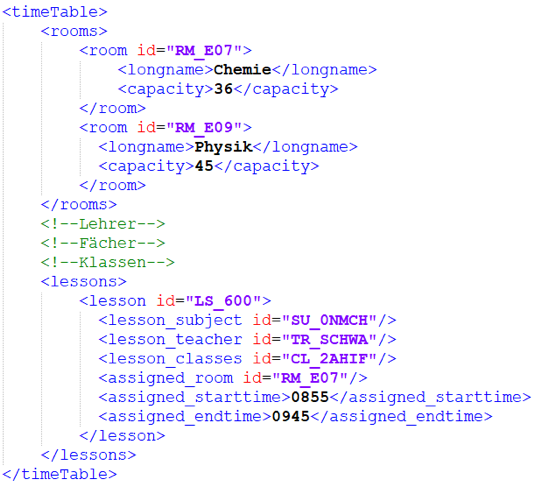
\includegraphics[width=0.3\textwidth]{Content/images/xml/xml.png}
    \end{center}
    \caption{Beispiel}
  \end{wrapfigure}
XML besteht aus sogenannten Tags, die zwischen zwei spitzen Klammern stehen. In XML können beliebig viele eigenen Tags definiert werden. In XML ist also lediglich definiert wie solche Tags auszusehen haben. Wenn ein Tag einen Bereich umschließt, dann gibt es einen öffnenden und einen schließenden Tag. Zwischen den Tags kann entweder nichts stehen, ein Text oder weitere Elemente. Das bedeutet, dass Tags ineinander verschachtelt werden können. Auf diese Weise kann eine Hierarchie erzeugt werden. Wenn der XML-Tag keinen Inhalt hat, kann er folgendermaßen alleinstehen. Bei Bedarf kann ein Tag außerdem einen oder mehrere Attribute haben. Die Syntax dazu sieht folgendermaßen aus. Attribute bestehen immer aus einem Namen und einem Wert. Der Wert wird mit doppeltem Anführungszeichen umschlossen und mit einem Gleichheitszeichen zugewiesen. 
Falls man Informationen speichern will, die nicht verarbeitet werden sollen, kann man Kommentare verwenden. Diese werden mit spitzen Klammern, Ausrufezeichen und Bindestrichen erstellt.

Um ein Dokument in XML zu schreiben, gelten ein paar allgemeine Formationsregeln. So muss jedes XML-Dokument wenigstens ein so genanntes Wurzel-Element enthalten, das allen anderen Elementen übergeordnet ist. Außerdem dürfen sich die Elemente nicht gegenseitig überschreiben. Beherzigt man diese Regeln beim Erstellen eines Dokuments, so spricht man von einem wohlgeformten XML-Dokument.
Bei der Erstellung eines gültigen XML-Dokuments kann man sich mit einigen online Validatoren abhelfen.

Um das ganze anhand eines Beispiels zu erklären habe ich das SYP-Projekt die Stundenplanverwaltung vom Stefan, Hofer und mir hergenommen. Hier haben wir eine XML-Schnittstelle implementieren müssen, um die Stundenpläne in unser Programm zu importieren. Um es besser erklären zu können habe ich das Beispiel etwas vereinfacht. Am Anfang des XML-Files haben wir Daten wir die Räume, Lehrer, Fächer oder die Klassen.
Wie man sieht sind die Tags Longname und Capacity hierarchisch dem Tag room untergeordnet und mit Hilfe von den Attributen kann man die Id der Rooms festlegen.

In der Datenbank würde das dann folgendermaßen abgebildet sein:
Diese Lehrer, Fächer, Klassen und Räume werden dann benötigt, um eine einzelne Unterrichtseinheit zu speichern. Hier sieht man anschließend auch noch wie Fremdschlüssel in XML darzustellen sind
Und in der Datenbank würde die Lesson dann folgendermaßen abgebildet sein:

\section{Vor und Nachteile}

Die wichtigsten Vorteile von XML sind die große Verbreitung und der geringe Lernaufwand der betrieben werden muss, bis man diese Datenformat beherrscht. Außerdem kann XML leicht von Menschen und Maschinen interpretiert werden.

Der einzige Nachteil von XML ist, dass eine in XML-gespeicherte Struktur viel Speicherplatz benötigen. Dementsprechend benötigt die Verarbeitung von Daten in XML viel Zeit.

\section{Einsatz}

Grundsätzlich kann XML zum Beschreiben, Speichern und Austauschen von Daten genutzt werden.
XML wird häufig verwendet, um Anwendungsdaten zu importieren bzw. exportieren. Ein Beispiel wäre die Stundenplanverwaltung.

Zuletzt sollte noch erwähnt werden, dass es für jede gängige Programmiersprache auch entsprechende Bibliotheken gibt, mit denen man XML lesen und schreiben kann. Damit erleichtert man sich die Arbeit mit XML-Daten. In unserer Stundenplanverwaltung haben wir Beispielsweise Dom4J verwendet.